\section{Εισαγωγή}

\subsection{Εισαγωγή: σκοπός του λογισμικού}
O σκοπός του συστήματος που υλοποιούμε είναι η δημιουργία μιας ενιαίας και εύκολης στη χρήση πλατφόρμας που ενθαρρύνει τη συνεργατική παρατήρηση τιμών πρατηρίων υγρών καυσίμων και παρέχει αυτές τις πληροφορίες δωρεάν σε κάθε χρήστη. Καθώς τα υγρά καύσιμα αποτελούν βασικό και απαραίτητο αγαθό της σύγχρονης δυτικής κοινωνίας θεωρείται αρκετά πιθανό το παραπάνω σύστημα να προσεγγίσει μεγάλο μέρος πληθυσμού γεγονός που θα ωφελήσει οικονομικά ένα ευρύ μέρος της κοινωνίας με την εύρεση καυσίμων σε χαμηλότερες τιμές.

\subsection{Επισκόπηση του λογισμικού}
\begin{figure}[H]
    \centering
    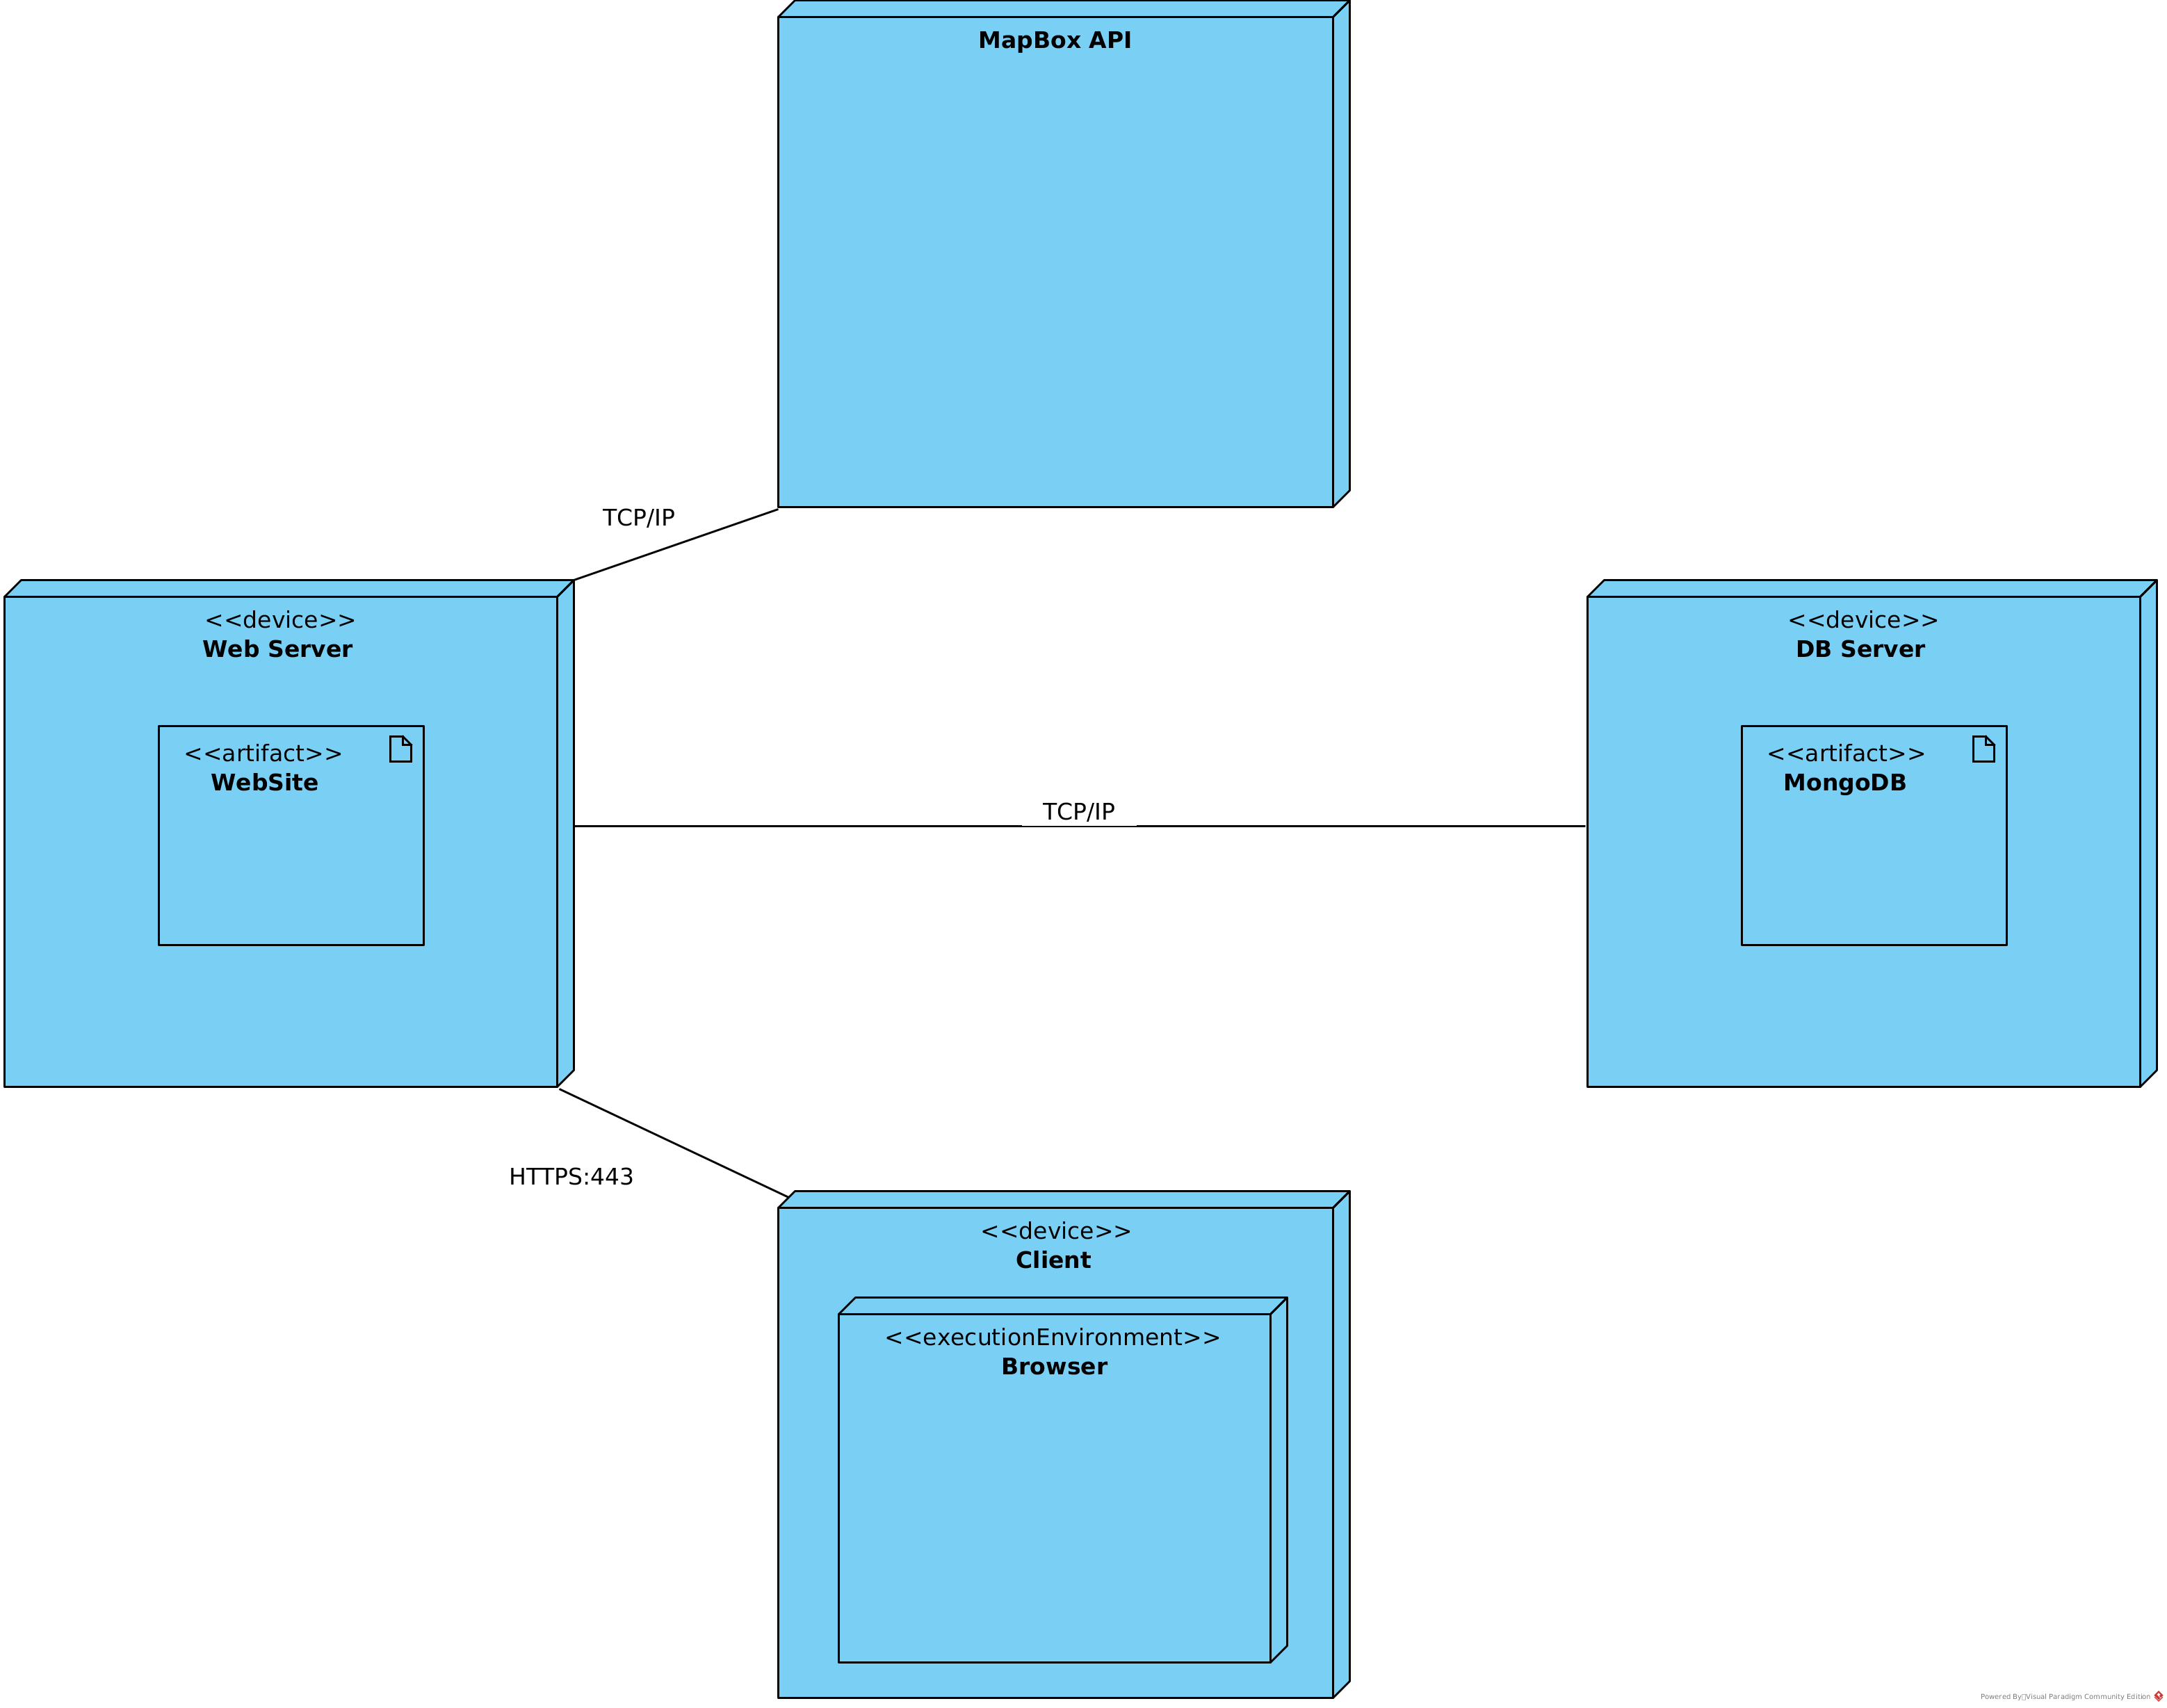
\includegraphics[width = \linewidth]{media/System/Deployment.png}
    \caption{Deployment Diagram}
\end{figure}

\subsection{Διεπαφές}
\subsubsection{Διεπαφές με εξωτερικά συστήματα και εφαρμογές λογισμικού}
Το μοναδικό εξωτερικό σύστημα που χρησιμοποιείται είναι το API του MapBox για τη χρήση του χάρτη και των λειτουργιών του. Η κλήση του API είναι ήδη προσαρμοσμένη στο Framework που χρησιμοποιείται, μέσω συγκεκριμένων κλάσεων και μεθόδων αυτών, αλλά χρειάζεται και η μεταφόρτωση δεδομένων από το API του MapBox.\\ \hfill \\
Η επικοινωνία μεταξύ του Frontend και του Backend γίνεται μέσω ενός REST API, το οποίο βοηθά στην παράλληλη εξέλιξη των δύο μέσω προδιαγραφών και μόνο. Αυτά γίνονται με HTTPS αιτήματα τύπου GET / POST / PUT / PATCH / DELETE.\\ \hfill \\
Επίσης, το Backend επικοινωνεί με τη βάση μας (MongoDB), μέσω DBMS statements τα οποία είτε παρέχονται έτοιμα από βιβλιοθήκη, είτε δημιουργήθηκαν από εμάς για πιο εξειδικευμένα queries. Έτσι, λαμβάνει τα απαραίτητα δεδομένα που ζητούνται μέσω του REST API.
\begin{figure}[H]
    \centering
    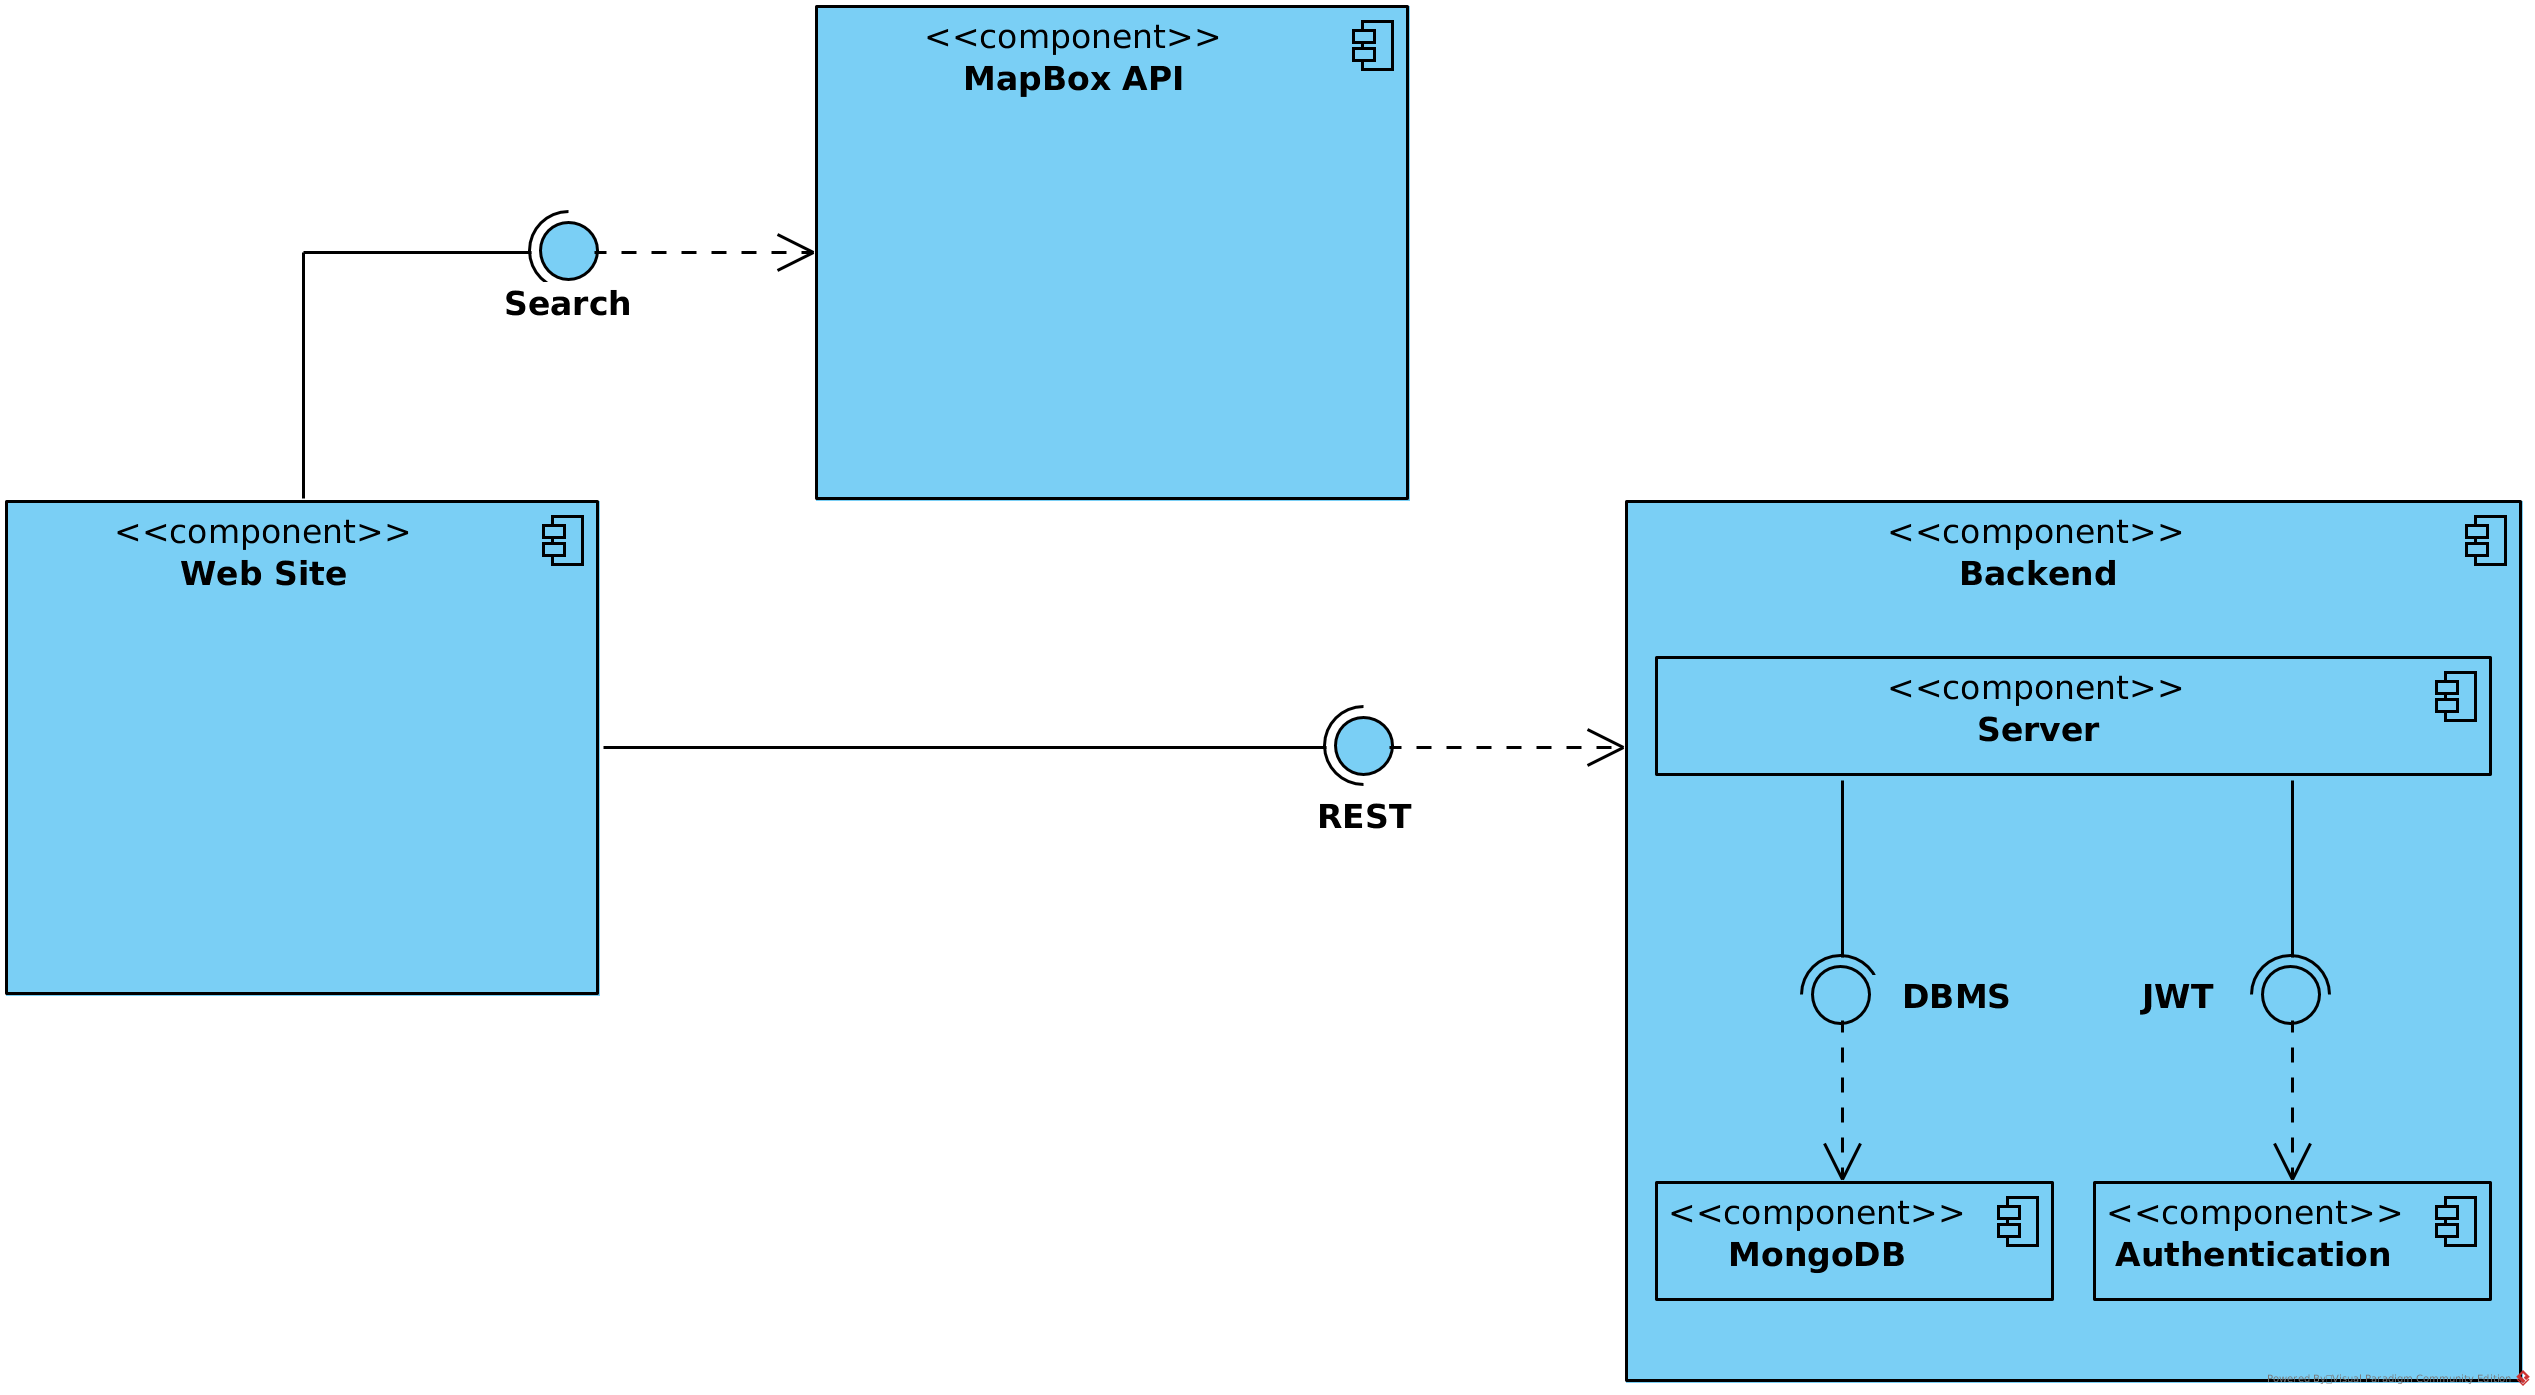
\includegraphics[width = \linewidth]{media/System/UI_Sys_Soft.png}
    \caption{Component Diagram}
    \label{fig:Component}
\end{figure}


\subsubsection{Διεπαφές με το χρήστη}



\begin{figure}[H]
    \centering
    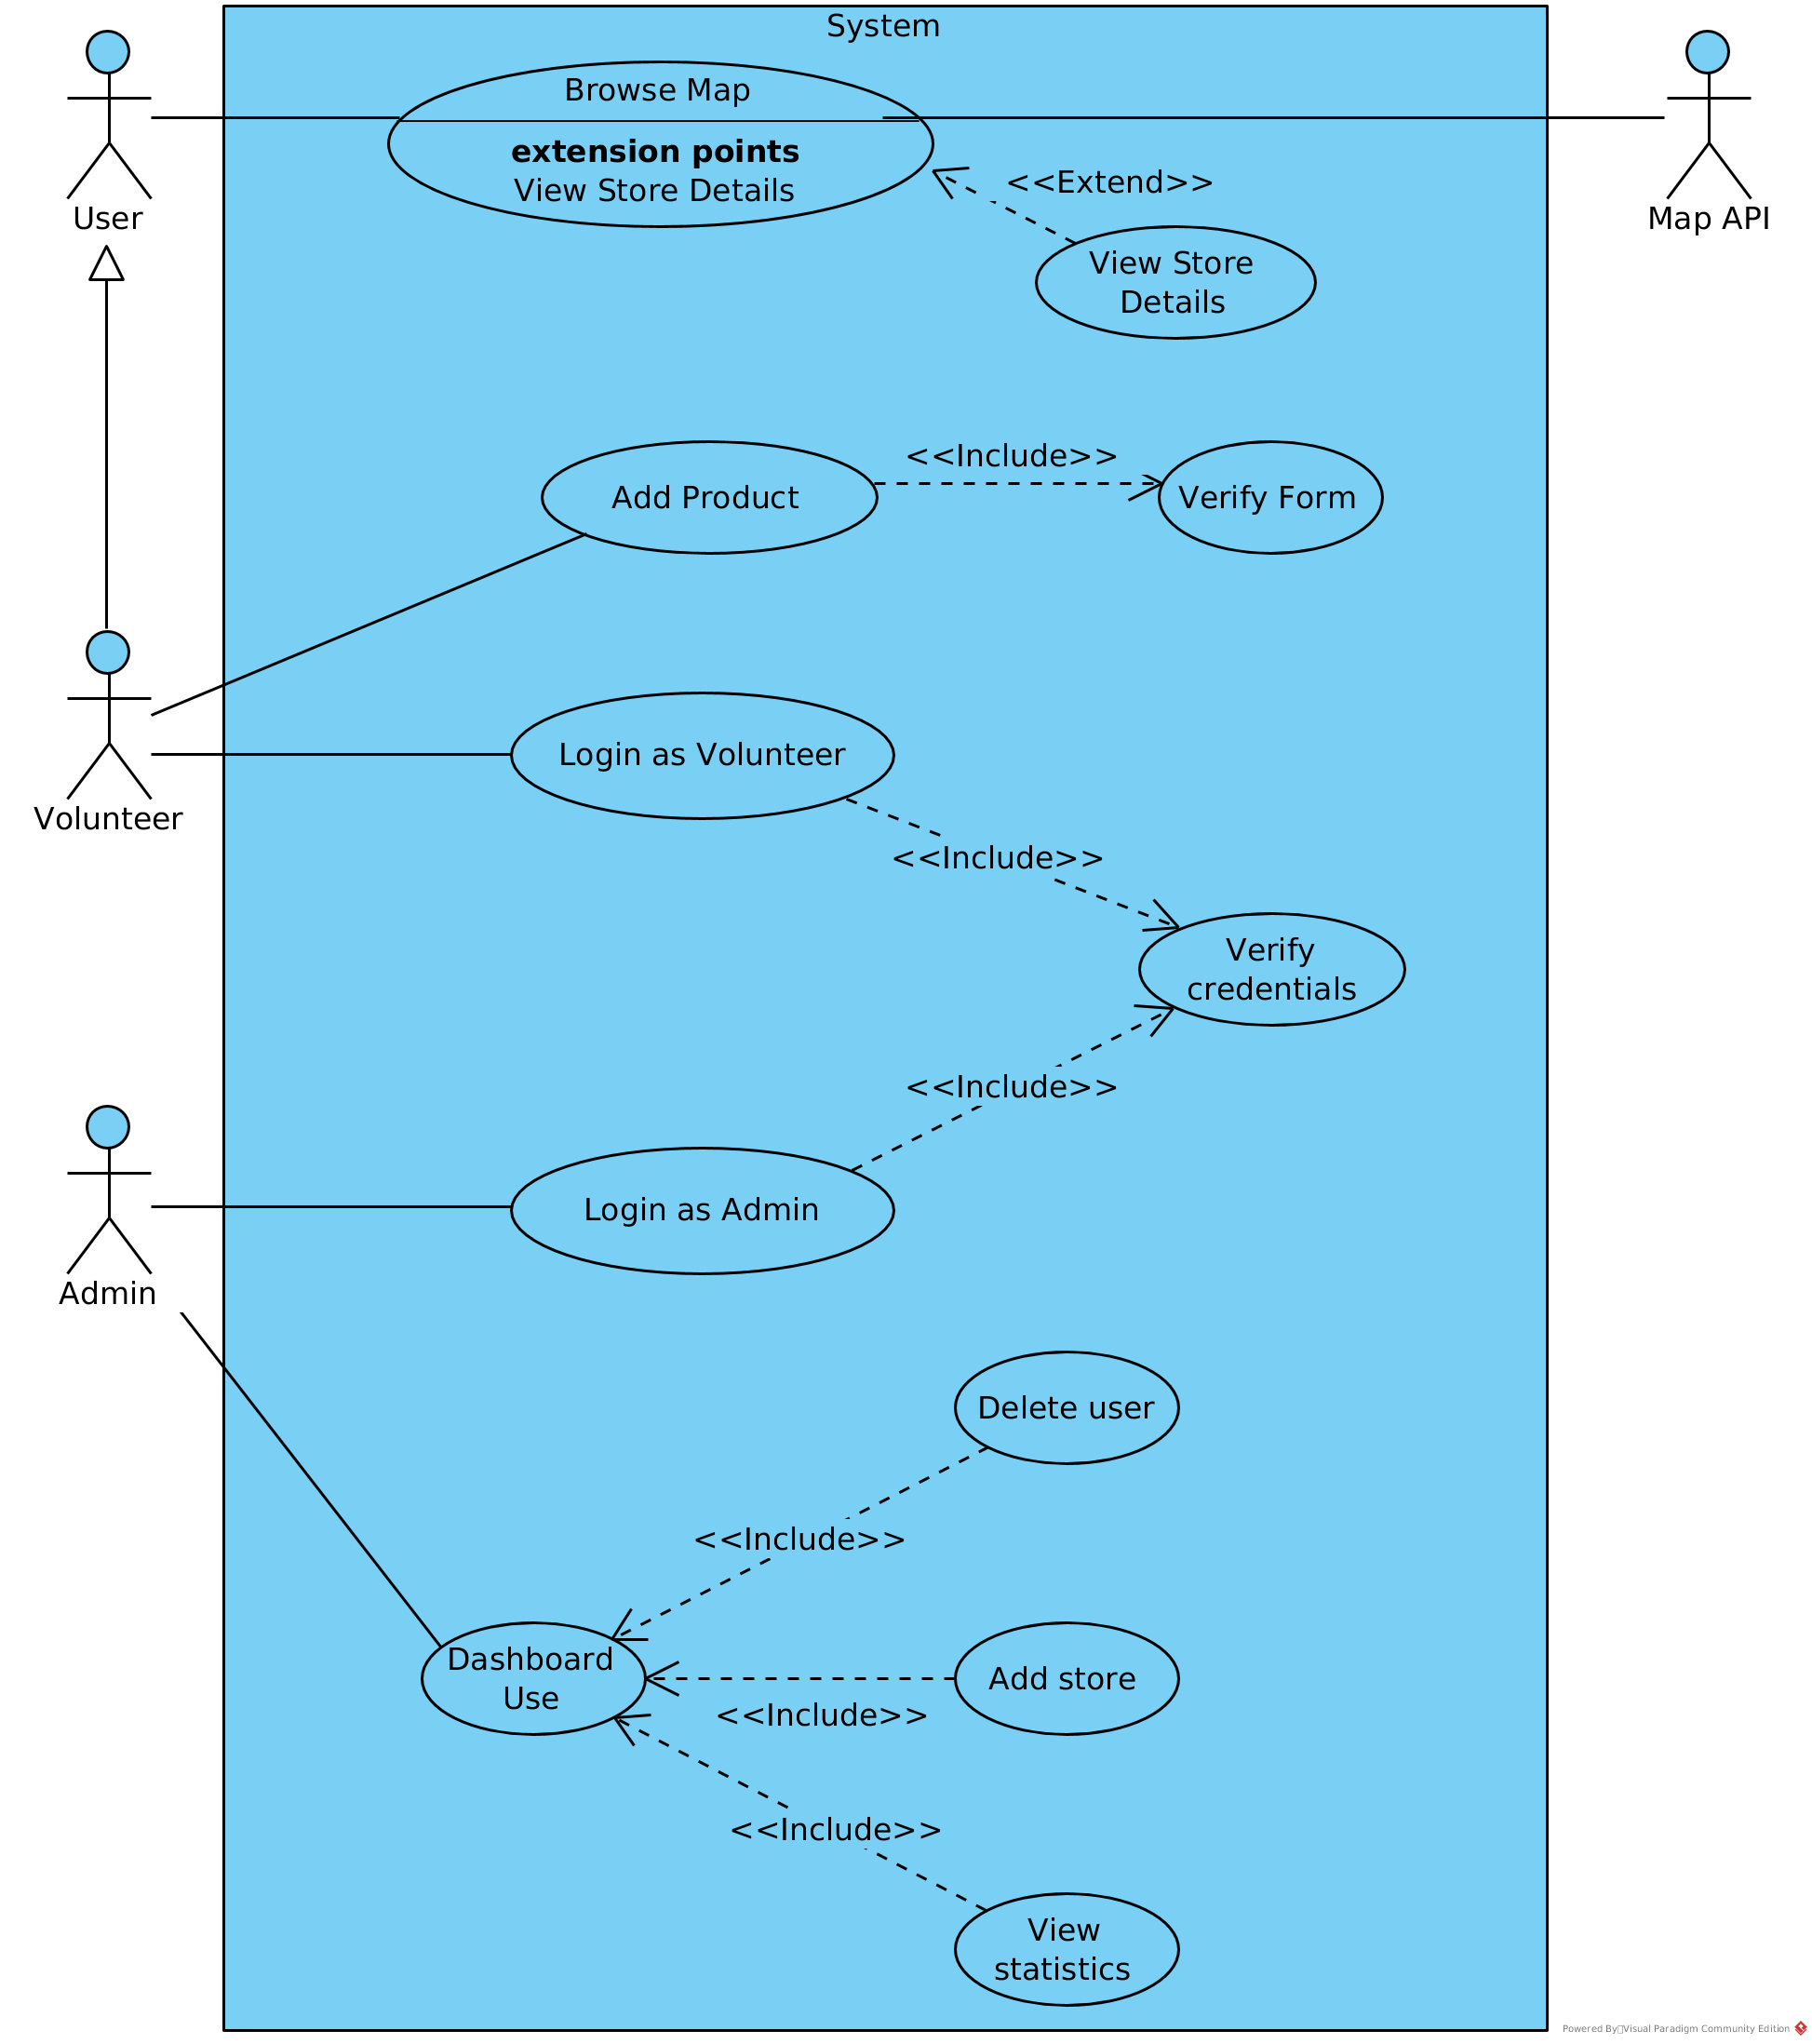
\includegraphics[width = \linewidth]{media/UseCase/User_UI.png}
    \caption{User UI}
    \label{fig:User_UI}
\end{figure}

% \subsection{Διεπαφές με υλικό}
% Προδιαγραφή διεπαφών με υλικό (εφόσον απαιτείται, πχ αναγνώστες κ.ά.)
% ΝΑ ΜΗΝ ΣΥΜΠΛΗΡΩΘΕΙ ΑΝ ΔΕΝ ΑΠΑΙΤΕΙΤΑΙ

% \subsection{Διεπαφές επικοινωνιών}
% Προδιαγραφή διεπαφών επικοινωνιών (αφορά στοιχεία λογισμικού που υλοποιούν τέτοιες διεπαφές, εφόσον
% υπάρχουν)
% ΝΑ ΜΗΝ ΣΥΜΠΛΗΡΩΘΕΙ ΑΝ ΔΕΝ ΑΠΑΙΤΕΙΤΑΙ